% \documentclass{book}

\documentclass[12pt]{article}
\usepackage[pdfborder={0 0 0.5 [3 2]}]{hyperref}%
\usepackage[left=1in,right=1in,top=1in,bottom=1in]{geometry}%
\usepackage[shortalphabetic]{amsrefs}%
\usepackage{amsmath}
\usepackage{enumerate}
\usepackage{enumitem}
\usepackage{amssymb}                
\usepackage{amsmath}                
\usepackage{amsfonts}
\usepackage{amsthm}
\usepackage{bbm}
\usepackage[table,xcdraw]{xcolor}
\usepackage{tikz}
\usepackage{float}
\usepackage{booktabs}
\usepackage{svg}
\usepackage{mathtools}
\usepackage{cool}
\usepackage{url}
\usepackage{graphicx,epsfig}
\usepackage{makecell}
\usepackage{array}

\def\noi{\noindent}
\def\T{{\mathbb T}}
\def\R{{\mathbb R}}
\def\N{{\mathbb N}}
\def\C{{\mathbb C}}
\def\Z{{\mathbb Z}}
\def\P{{\mathbb P}}
\def\E{{\mathbb E}}
\def\Q{\mathbb{Q}}
\def\ind{{\mathbb I}}

\graphicspath{ {images14/} }

\begin{document}

\section*{1 May 2017}

\subsection*{Time Stepping}

\subsubsection*{Scheme}
Now that we have successfully constructed double pulses, we will do numeric time-stepping to examine the behavior of double pulses which start near the stationary double pulse solutions. For this, we use the 5th order KdV written in a moving frame with speed $c$.
\[
u_t = u_{xxxxx} - u_{xxx} + c u_x - 2 u u_x
\]
We write this as
\[
u_t = Lu + F(u)
\]
where $L = \partial_x^5 - \partial_x^3 + c \partial_x$ is the linear part of the RHS, and $F(u) = -2 u u_x$ is the nonlinear part.\\

For the numerical scheme, it turns out that (explicit) RK4 is not stable. Because of the nonlinear part, a purely implicit scheme does not make sense. Thus we use a IMEX (splitting) scheme. Since we used it successfully in APMA 256 for the 3rd order KdV equation, we choose Crank-Nicoloson/Adams-Bashforth 2 as our IMEX scheme. This works better than the 1st ordet Euler Forward/Euler Backward scheme. There are likely much better schemes for this, but this appears to work. For the spatial operators, we use Fourier spectral methods with periodic BCs as before. The scheme is:

\[
\frac{u^{n+1} - u^n}{k} = \frac{3}{2}F(u^n) - \frac{1}{2}F(u^{n-1}) + \frac{1}{2}\left(Lu^{n+1} - Lu^n \right) 
\]

where $u^n$ represents the $n$th time step, and $k$ is the time step size. For most of what we will do, a time step size of 0.01 seems to work well. In general, we use $N = 256$ spatial grid points (Fourier nodes) and a domain size of $L = 25$.

\subsubsection*{Intial Conditions and Initial Tests}
First we tested out numerical scheme using our constructed double pulses as initial conditions. These should be stationary solutions, so they should not change with timestepping. This is indeed the case. The double pulse maintains its shape throughout timestepping. A very small amount of translation occurs, which I am attributing to numerical error.\\

Now we modify our double pulse and see what happens. There are many ways we can do this. Here are some that don't do what we want.

\begin{enumerate}

	\item Keep the double pulse as is, and change $c$ slightly. If the double pulse is a stationary solution with speed $c_0$, all this does is give us a solution which translates with speed $|c - c_0|$. All we have done is change the speed of the moving frame.
	\item Modify the pulse heights. We can either scale the whole thing by a small amount or add small bumps (e.g. Gaussians) to the peaks. Either way, this gives us a double pulse which translates to the L or R but remains roughly intact. This is not surprising since for stationary solutions there is a nice linear relationship between the speed $c$ and the peak height.
	\begin{figure}[H]
		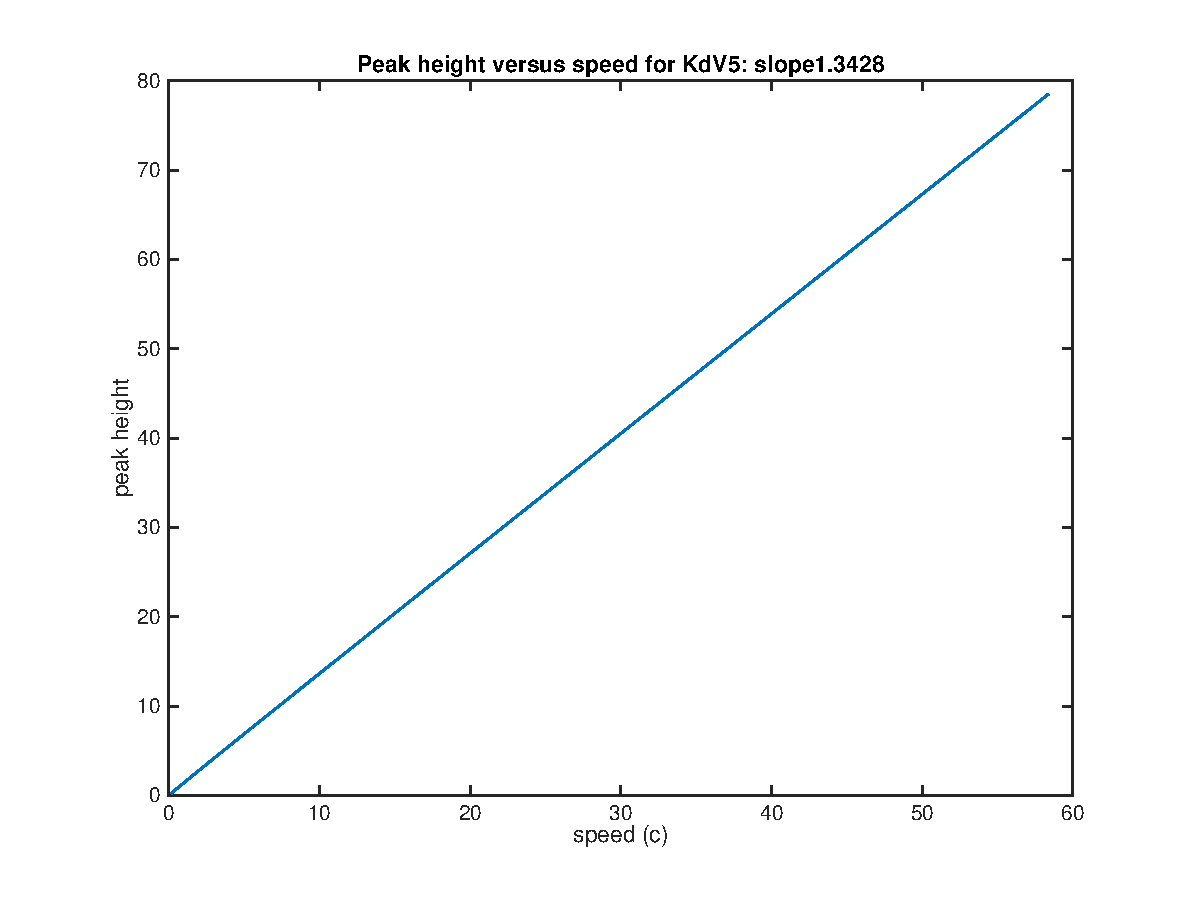
\includegraphics[width=8.5cm]{peakheights.eps}
	\end{figure}
	So as long as we don't make too big a change, this essentially produces a double pulse which is roughly a stationary solution but has different speed $c$. 

\end{enumerate}

From this, we learn that we need to keep the speed $c$ and the peak heights the same. The logical thing to try next is to change the distance between the two pulses. We start with a crude approach, mostly because it is easy to code.

\begin{enumerate}
	\item To increase distance between the pulses, take the value of the center gridpoint, i.e. at $x = 0$ and duplicate it for one gridpoint to the L and to the R of center, shifting the L and R pieces outward to accommodate. This gives us a double pulse which is still even, and the piece in the middle is still flat. We can keep repeating this to increase separation between pulses.
	\item To decrease distance between the pulses, we basically do the same thing, except we remove points in the center and shift the L and R pieces inward.
\end{enumerate}

\subsubsection*{Double Pulse 2}
Here we start with ICs near the double pulses we think are stable, i.e. the ones with eigenvalues which are purely imaginary (or at least the numerics suggest this is true). We use speed $c = 9.4812$ since we have constructed two stable double pulses for this value of $c$. We first look at Double Pulse 2.\\

First, we widen by two gridpoints on each side (0.3906 on each size, since we use $N = 256$ gridpoints on $[-25, 25]$). Running for 5000 time steps, we get the following:

\begin{figure}[H]
	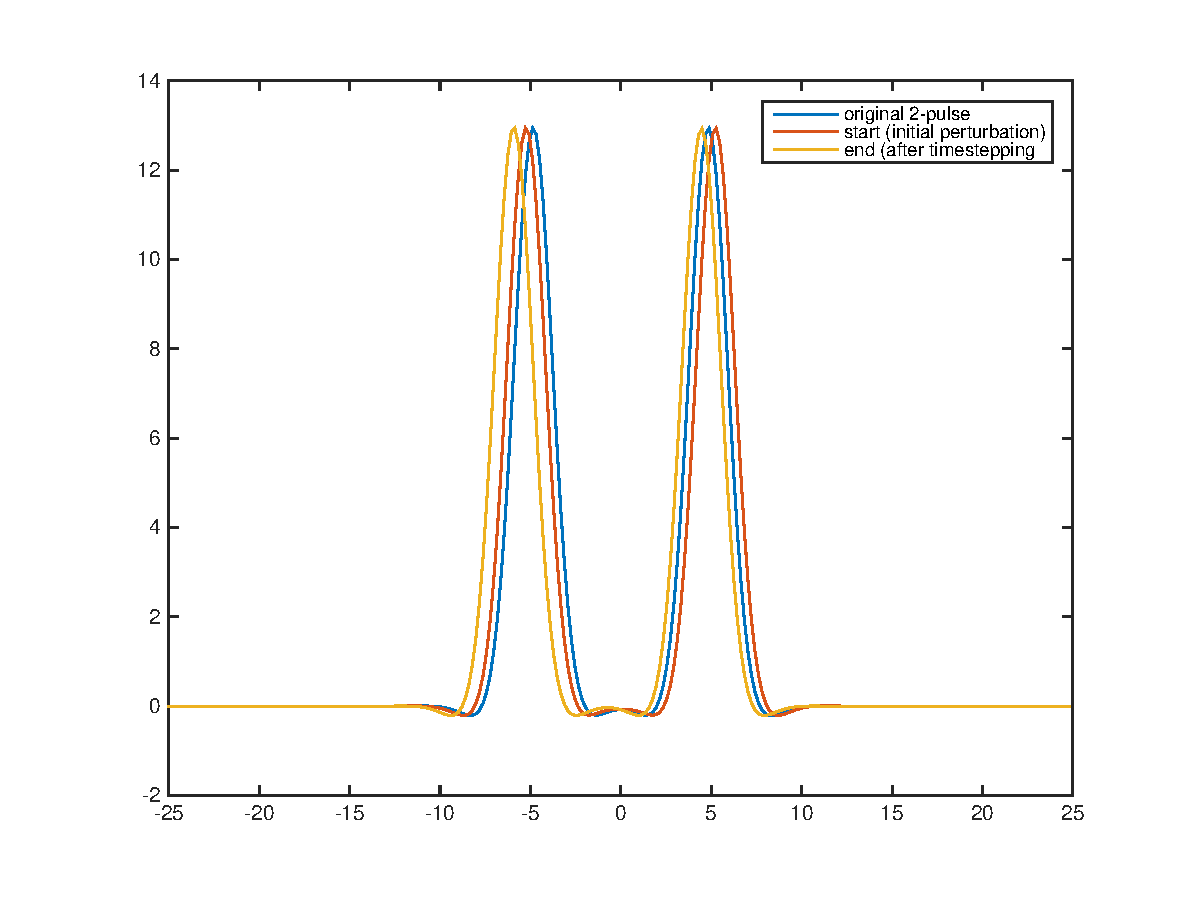
\includegraphics[width=8.5cm]{2double1a_t5000.eps}
\end{figure}

It looks like we have translated a bit to the left, but that's it. Since we are hoping the stable double pulse is a nonlinear center, let's look at the distance between peaks as time is varied. Since space is discretized, this is not continuous.

\begin{figure}[H]
	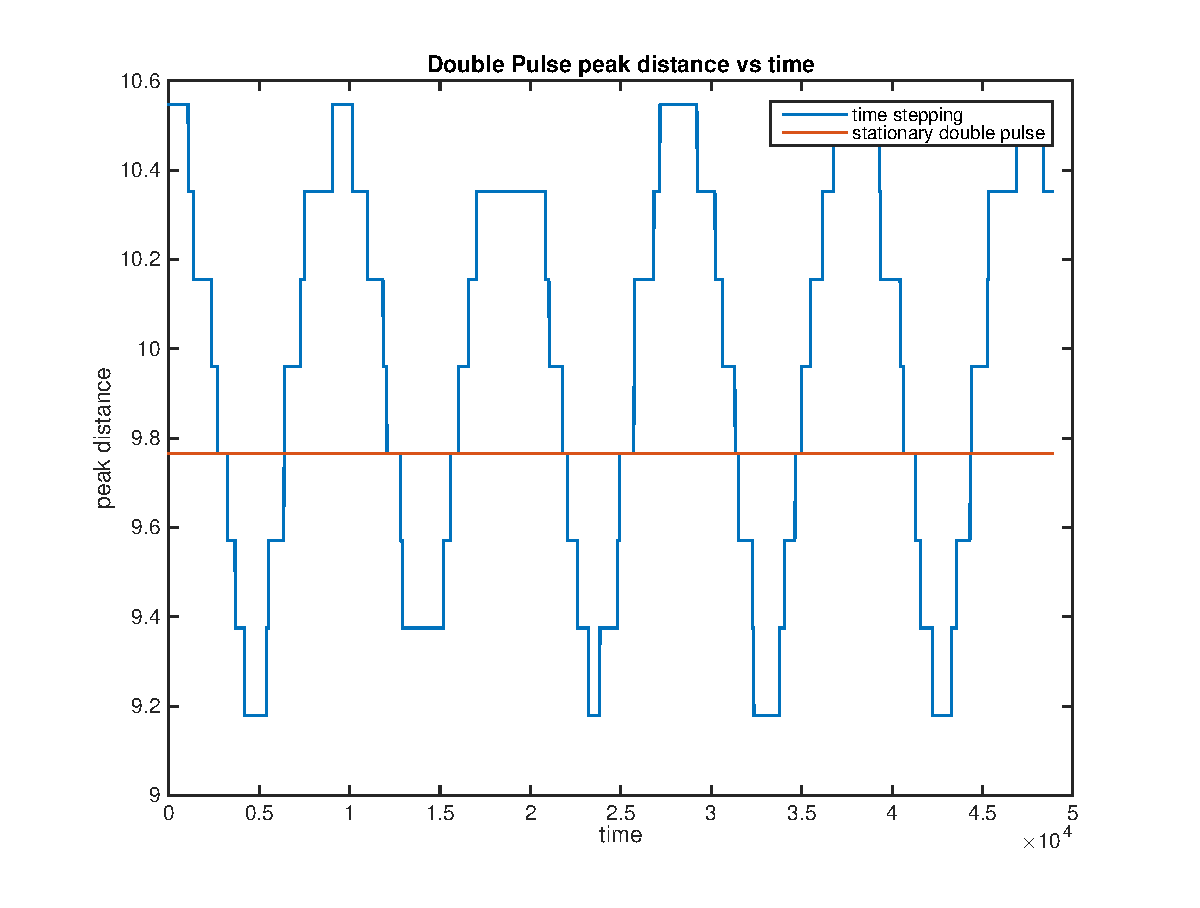
\includegraphics[width=8.5cm]{2double1a_osc1.eps}
\end{figure}

The peak distance oscillates periodically, and oscillations occur about the peak distance of the stationary double pulse (the center equilibrium point; it's not in the middle but that's okay). This is what we were hoping for. If use take more grid points, we can see this better. This is for the same starting peak distance as the case with 256 grid points.

\begin{figure}[H]
	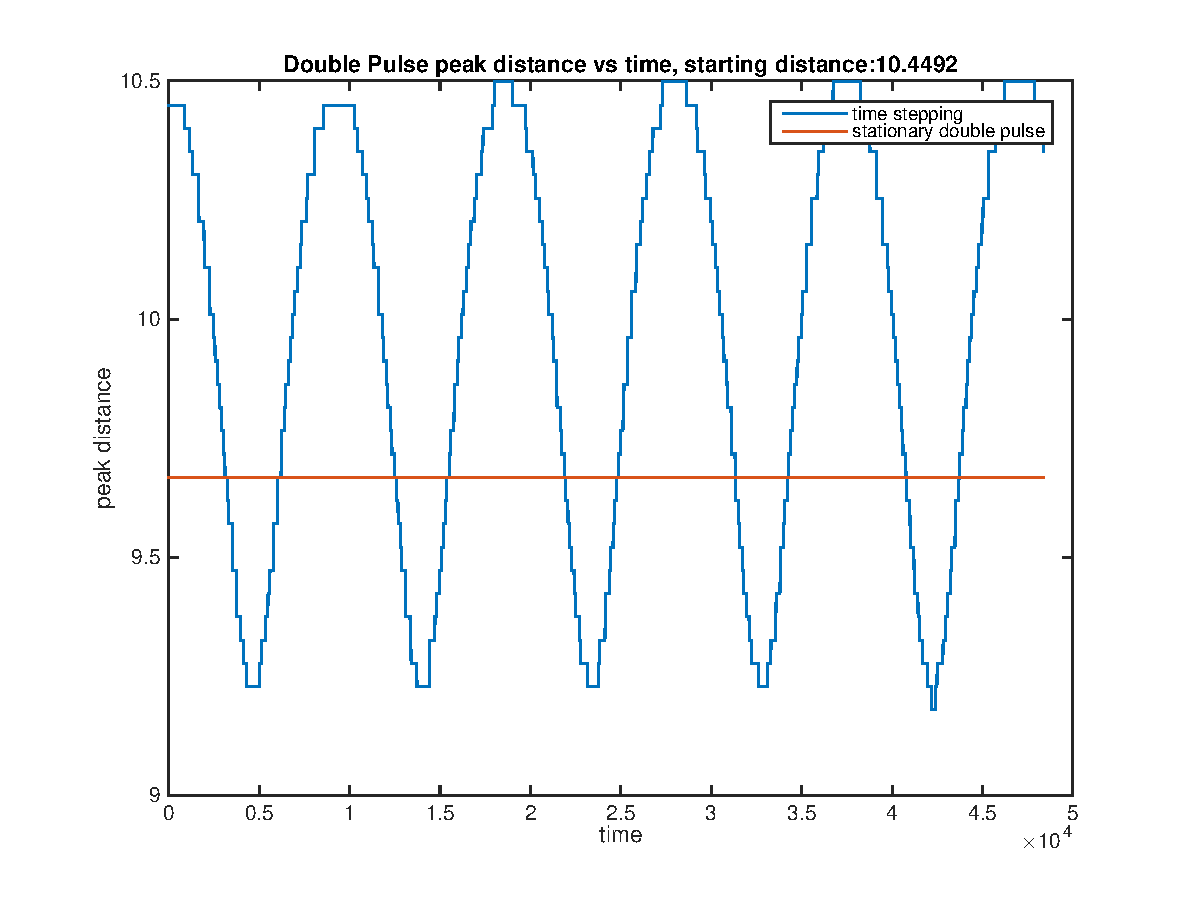
\includegraphics[width=8.5cm]{2double1a_osc1_1024.eps}
\end{figure}

We can also experiment with different starting peak distances. Here we do one narrower and one wider.

\begin{figure}[H]
	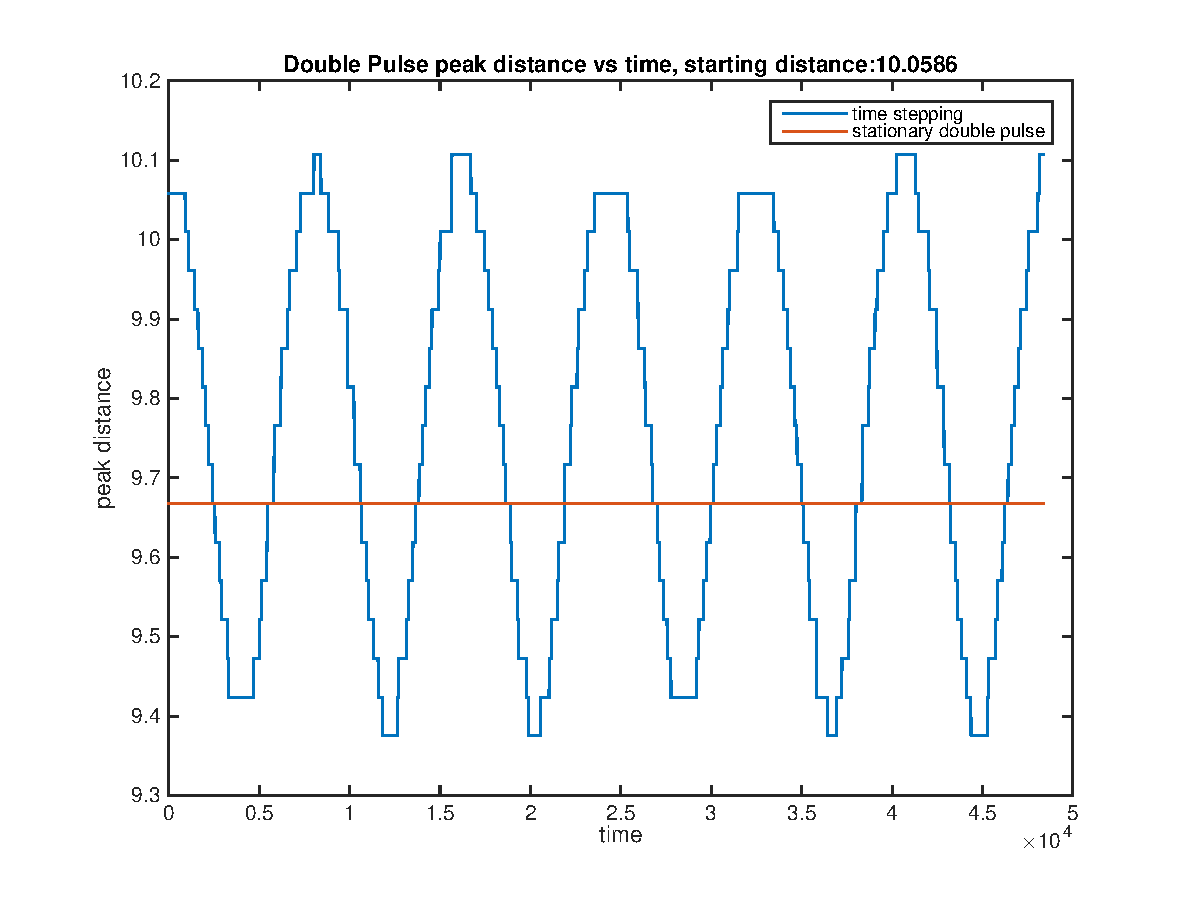
\includegraphics[width=8.5cm]{2double1a_osc2_1024.eps}
	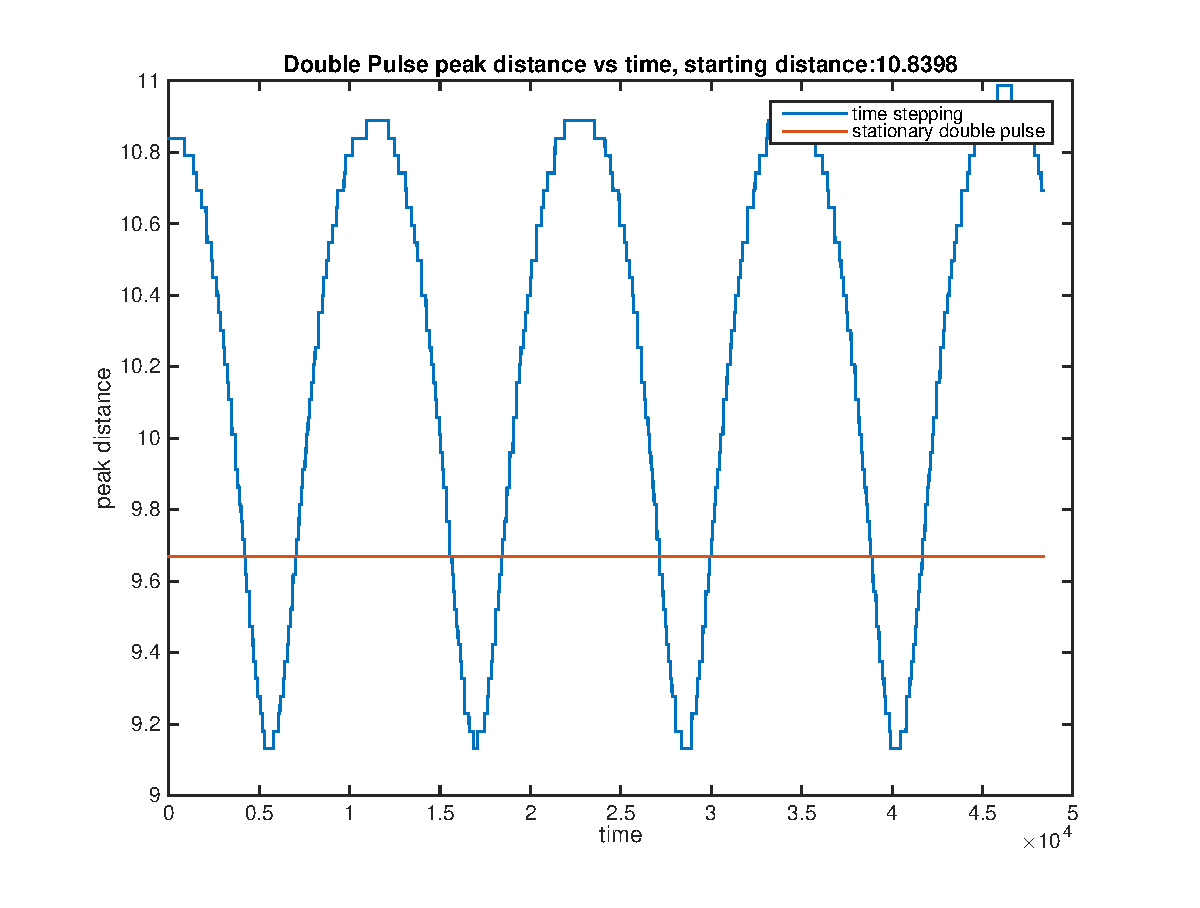
\includegraphics[width=8.5cm]{2double1a_osc3_1024.eps}
\end{figure}

From this, we see that narrow oscillations are faster. I'm not sure what I expected this to be, but it at least makes physical sense to me.

\subsubsection*{Double Pulse 4}
We repeat this for Double Pulse 4. Since the oscillations are slower, we run for 100000 time steps. We only do this for $N=256$ grid points since it takes too long otherwise. We observe the same pattern of oscillations as for Double Pulse 4. 

\begin{figure}[H]
	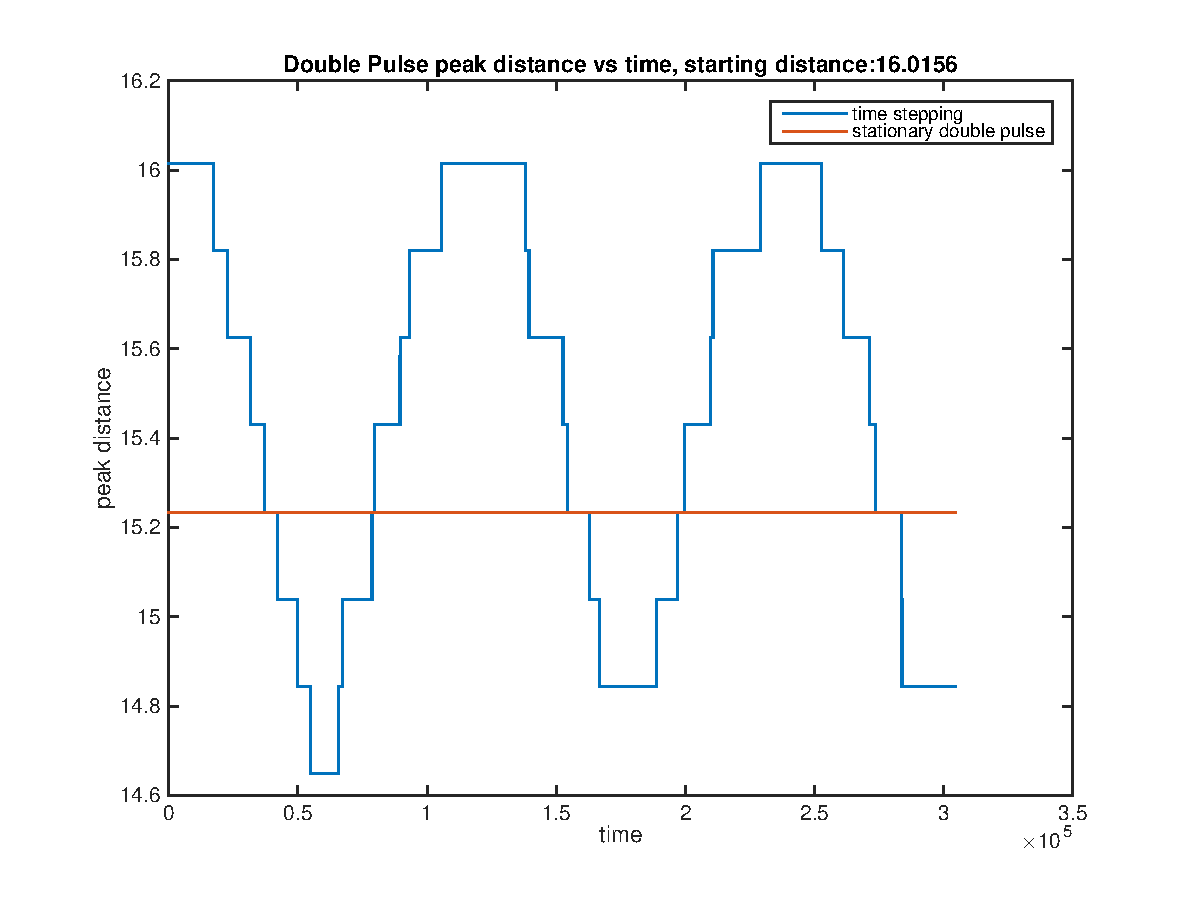
\includegraphics[width=8.5cm]{2double2a_osc1_1024.eps}
\end{figure}

\subsubsection*{Double Pulse 1}
Now let's see what happens for the unstable pulses, i.e. the ones which have a positive eigenvalue. Again, we increase the distance between the pulses and use that for the initial condition. Here are plots of the timestepping for four initial conditions.

\begin{figure}[H]
	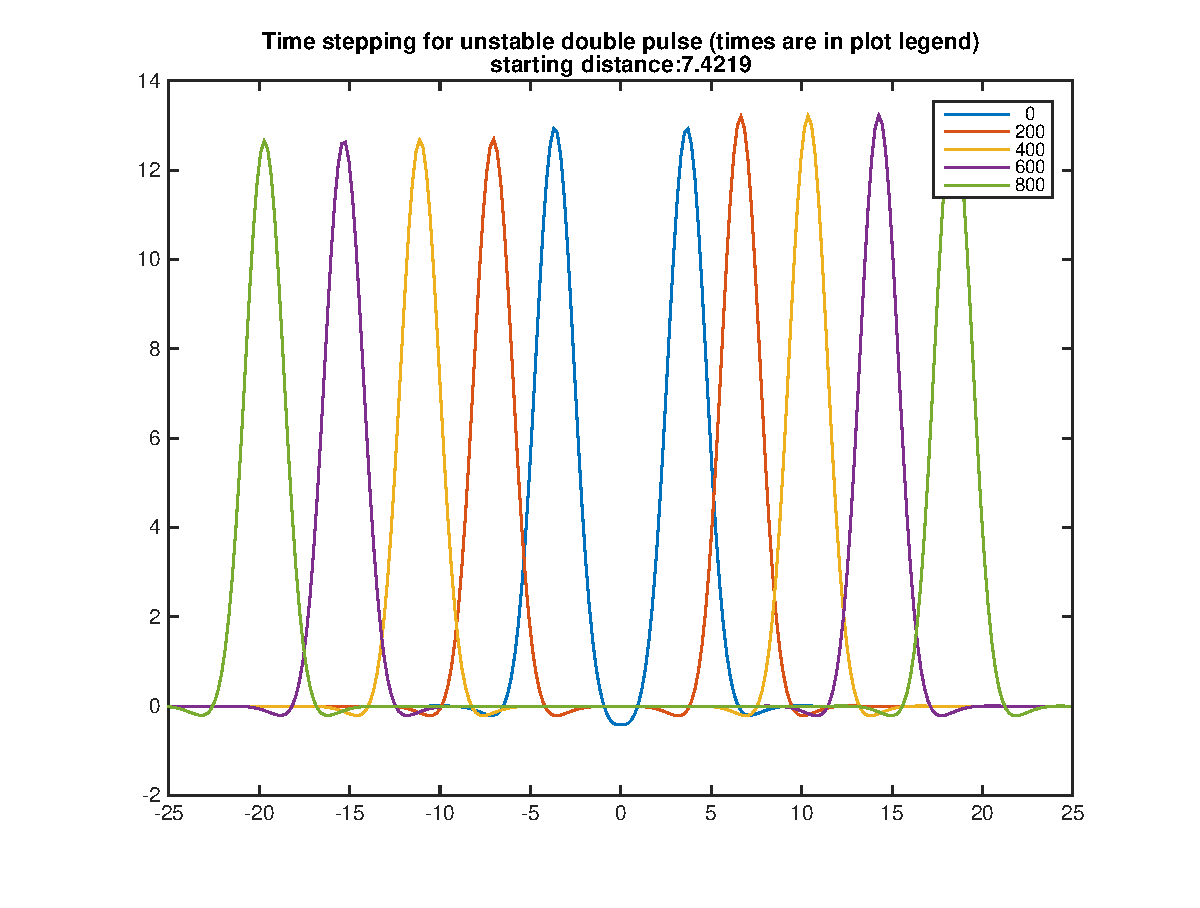
\includegraphics[width=8.5cm]{2double1_dist1.eps}
	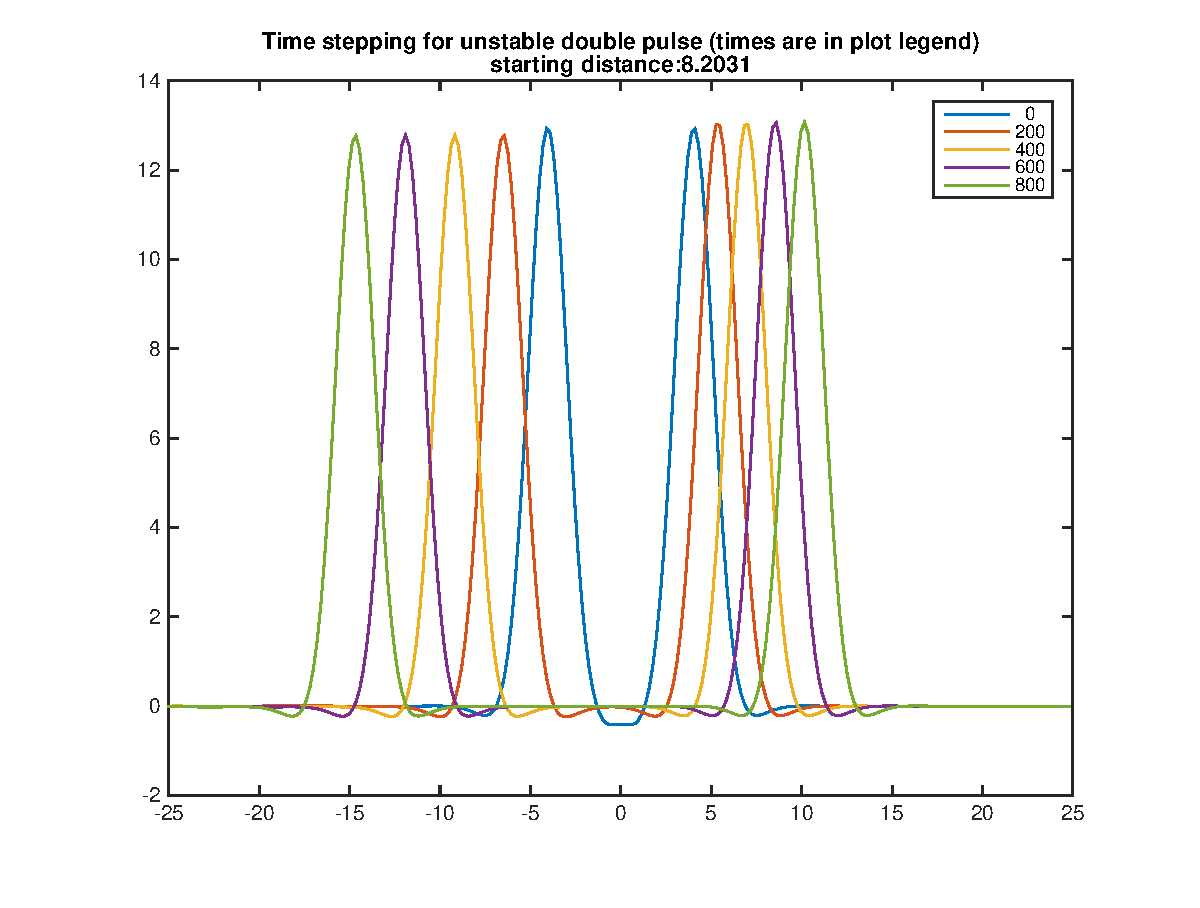
\includegraphics[width=8.5cm]{2double1_dist2.eps}
\end{figure}
\begin{figure}[H]
	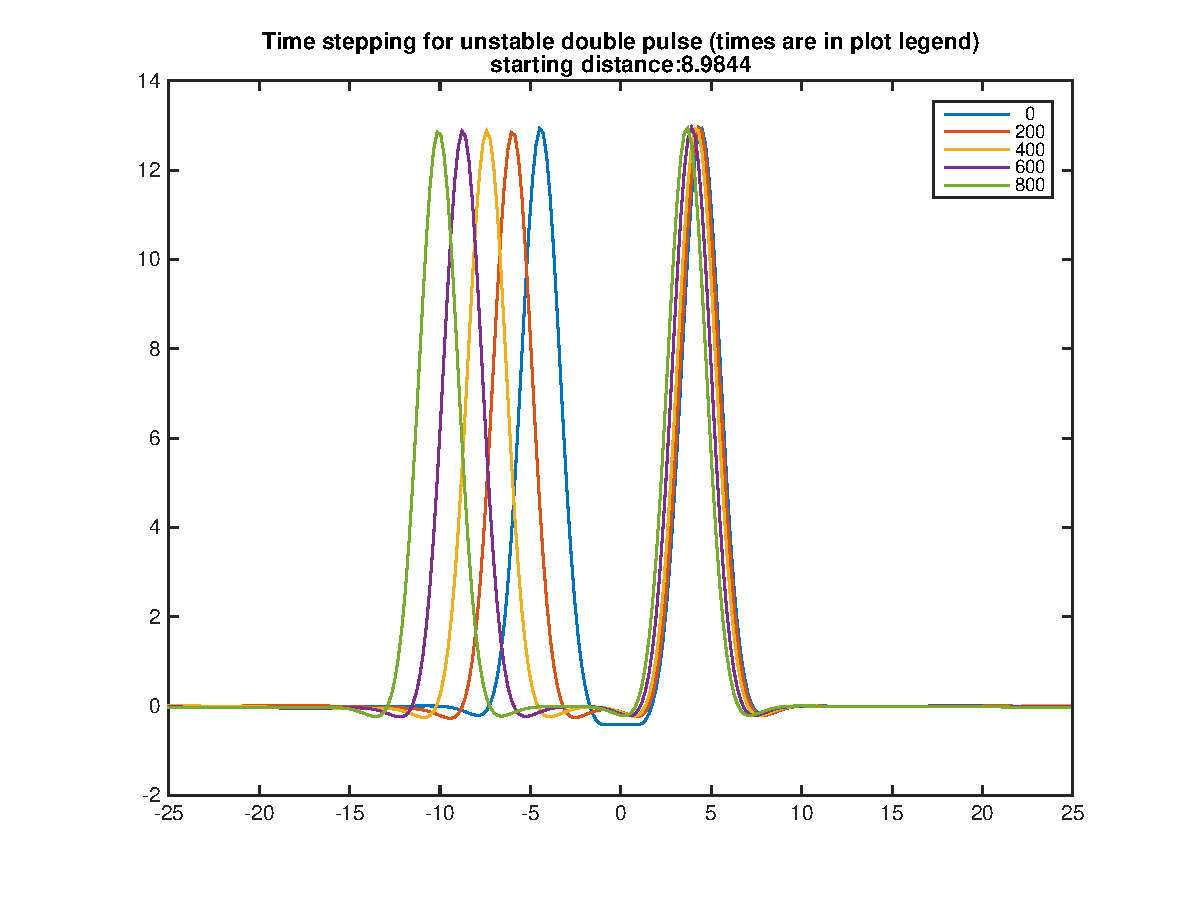
\includegraphics[width=8.5cm]{2double1_dist3.eps}
	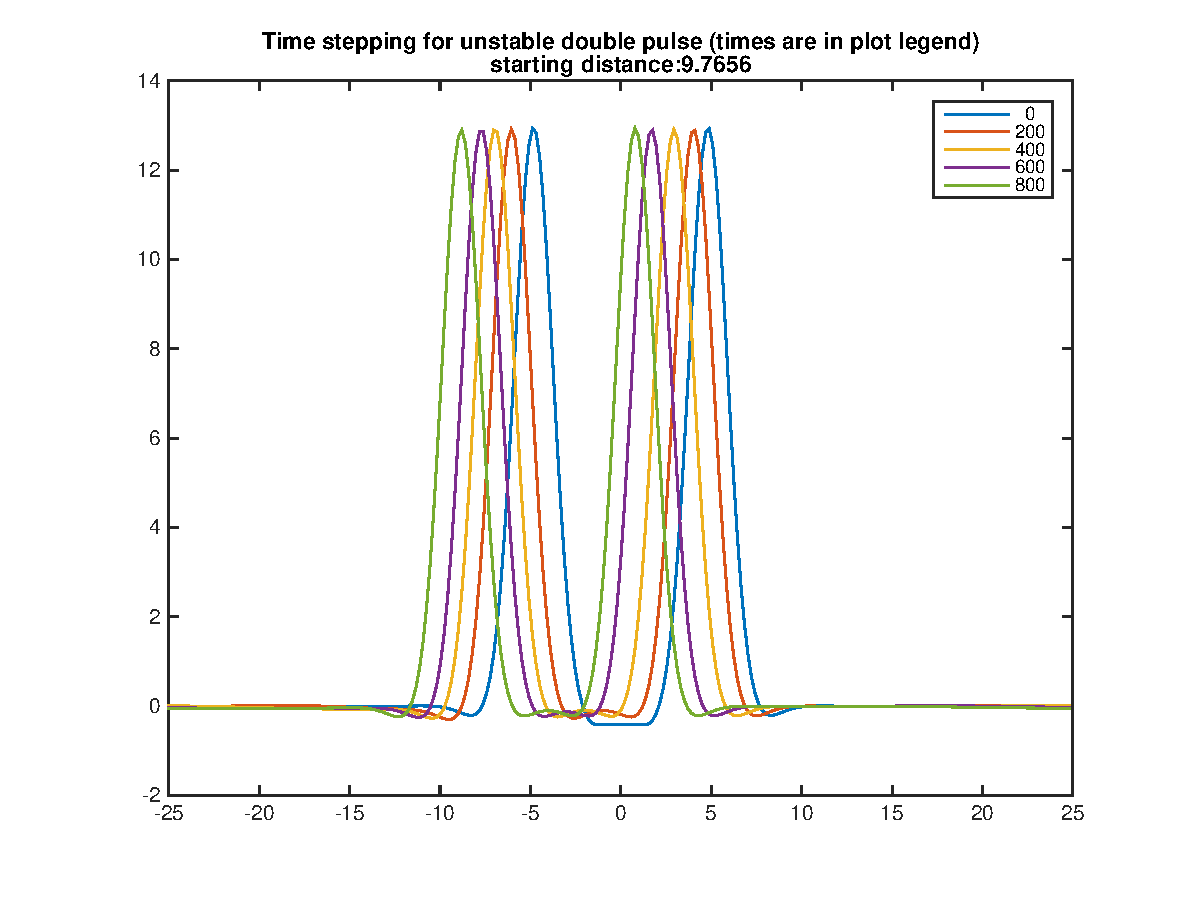
\includegraphics[width=8.5cm]{2double1_dist4.eps}
\end{figure}

For the first two, the double pulse heights become uneven (one shorter, one taller) and the two pulses move in opposite directions. This is most pronounced for the first one (smallest starting distance). In the second, the left pulse moves left faster, while the right pulse moves right slower. This is even more pronounced in the third one, where the left pulse moves left, but the right pulse is almost stationary. In the fourth one, both pulses move to the left with approximately the same speed, and the profile looks like a slightly distorted version of Double Pulse 2.\\

The most interesting case the fourth one, where we look like a traveling, slightly distorted version of Double Pulse 2. Let's plot the distance between peaks as a function of the time step. I stop this at 3500 time steps, because around then the peaks wrap around the periodic boundary. At some point, the numerics for this break down.

\begin{figure}[H]
	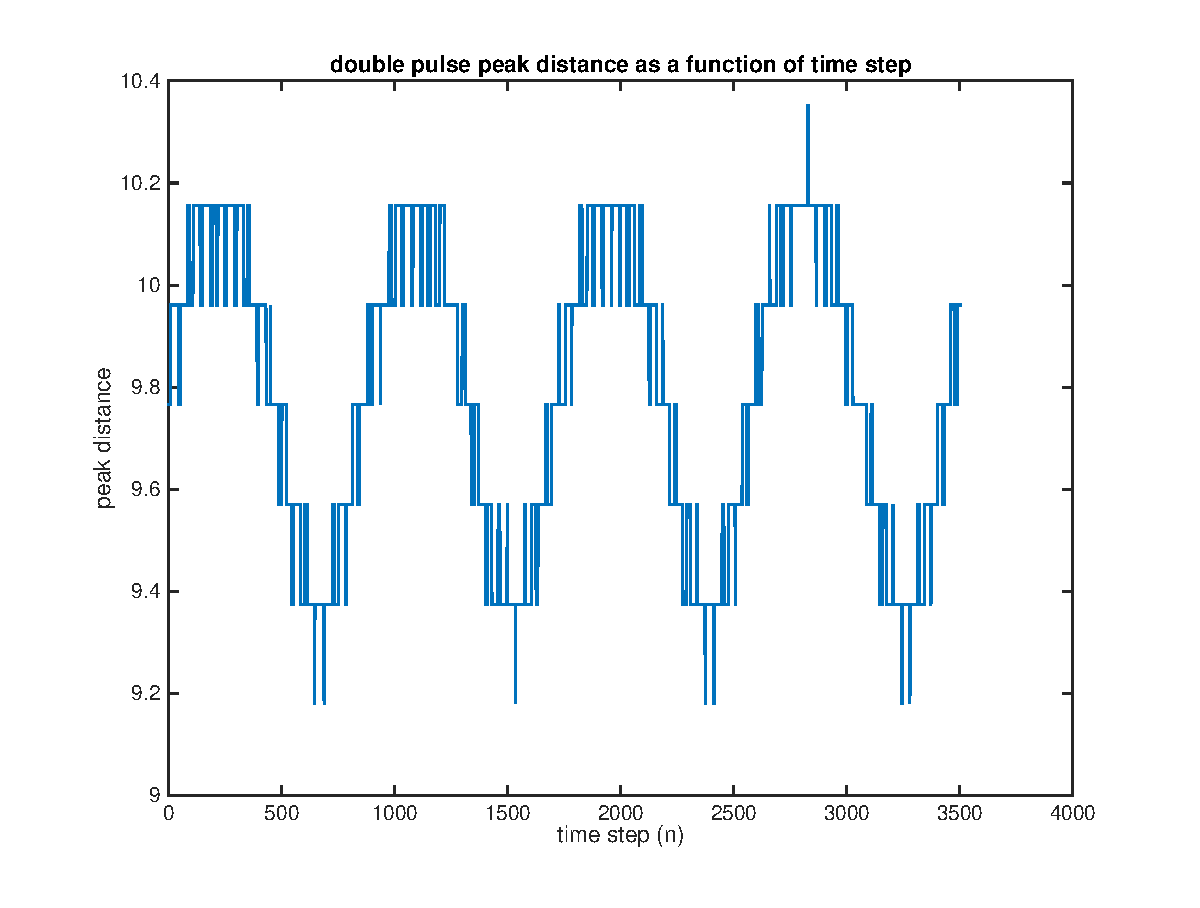
\includegraphics[width=8.5cm]{2double1_osc1.eps}
\end{figure}
We see oscillations here, just as we did with Double Pulse 2. The peak distance for Double Pulse 2 (a little less than 9.7) lies between the extremes of these oscillations, which suggests that this initial condition may be captured by the (hypothesized) center around Double Pulse 2.

\section*{1 May 2017}

\subsection*{Time Stepping, continued}

Here we continue our time-stepping experiments. We considered three schemes:
\begin{enumerate}
	\item Crank-Nicolson / Adams-Bashforth 2 (IMEX): described and used above
	\item Crank-Nicolson (purely implicit): Since there is a nonlinearity, we have to use Newton's method to solve instead of just inverting a matrix once. Ends up being too slow, and no real improvement over the IMEX method. 
	\item Runke-Kutta 4 with integrating factor in Fourier space. This is a standard method used for KdV3. Taking the Fourier transform of the PDE, we get:
	\[
	\hat{u}_t = i(k^5 + k^3 + kc)\hat{u} - ik\widehat{u^2}
	\] 
	Letting $A = i(k^5 + k^3 + kc)$, this becomes:
	\[
	\hat{u}_t - A\hat{u} = - ik\widehat{u^2}
	\]
	Multiplying by integrating factor $e^{-At}$, we obtain
	\[
	\frac{d}{dt}\left(e^{-At}\hat{u} \right) = -ik e^{-At} \widehat{u^2}
	\] 
	Then we itererate this with RK4 (in Fourier space), using IFFT and FFT to compute $\widehat{u^2}$. Although this works, the time step required for stability is of order $1/N^2$, where $N$ is the number of Fourier nodes. This small time step is too impractical for long term integration.
\end{enumerate}

The IMEX method appears to be the most practical for long-time integration, so we will use that one. First, we look 
at long time integration. For our starting condition, we take our stable solution for Double Pulse 2 and stretch in the center by two grid points on each side of the middle, as described above. Distances between the peaks are computed after fitting with a cubic spline, and this is plotted versus time. Two plots are show below. In the first, we integrate to time 10000 (1e6 time steps), sampling every 1000 steps. In the second, we integrate to time 1000, sampling every 5 time steps.

\begin{figure}[H]
	\includegraphics[width=8.5cm]{every1000.pdf}
	\includegraphics[width=8.5cm]{every5.pdf}
\end{figure}

From these this appears to be a stable periodic orbit. In the first plot, the peak/trough heights look like they are fluctuating a bit, we are sampling only every 1000 time steps. When we sample more often, this difference essentially goes away, and the plot looks like more-or-less uniform oscillations. As a check, let's look at a graph of energy vs. time. Since for KdV5, the L2 norm is conserved, we will use that for the energy. Here is a graph of the L2 norm vs time for the longest time integration.

\begin{figure}[H]
	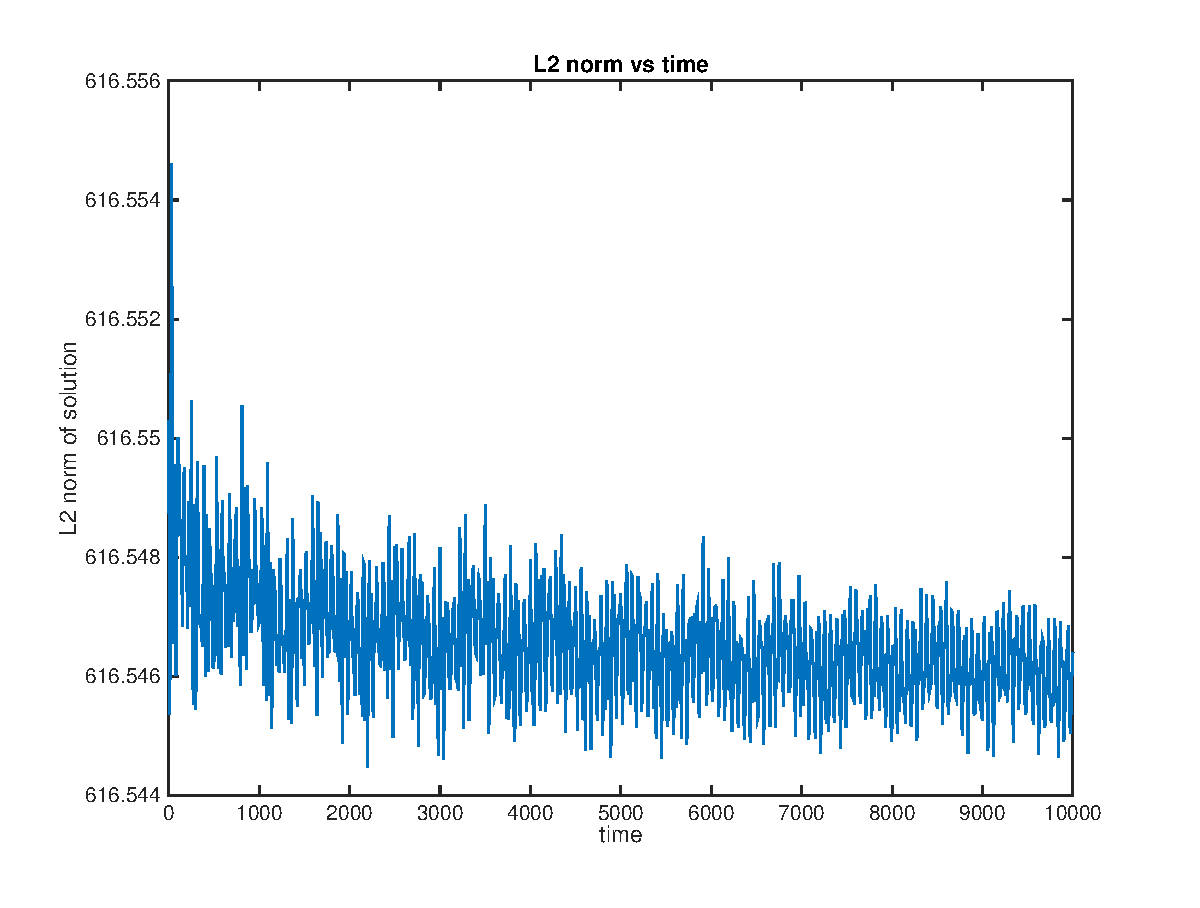
\includegraphics[width=8.5cm]{L2normvstime.eps}
\end{figure}
Any downward trend here is minimal. If we take the difference between the max and min of the L2 norm, and divide by the mean of the L2 norms, we get 1.6439e-05, which is very good for 1 million time steps.

\subsection*{Phase Portraits}

What we want to do now is plot the derivative of the peak distance (peak distance velocity) versus the peak distance to get a 2D phase portait (like we do in, say, the pendulum). One way to do this is just to take the derivative using finite differences. Below we have peak distance vs time and derivative of peak distance vs time.
\begin{figure}[H]
	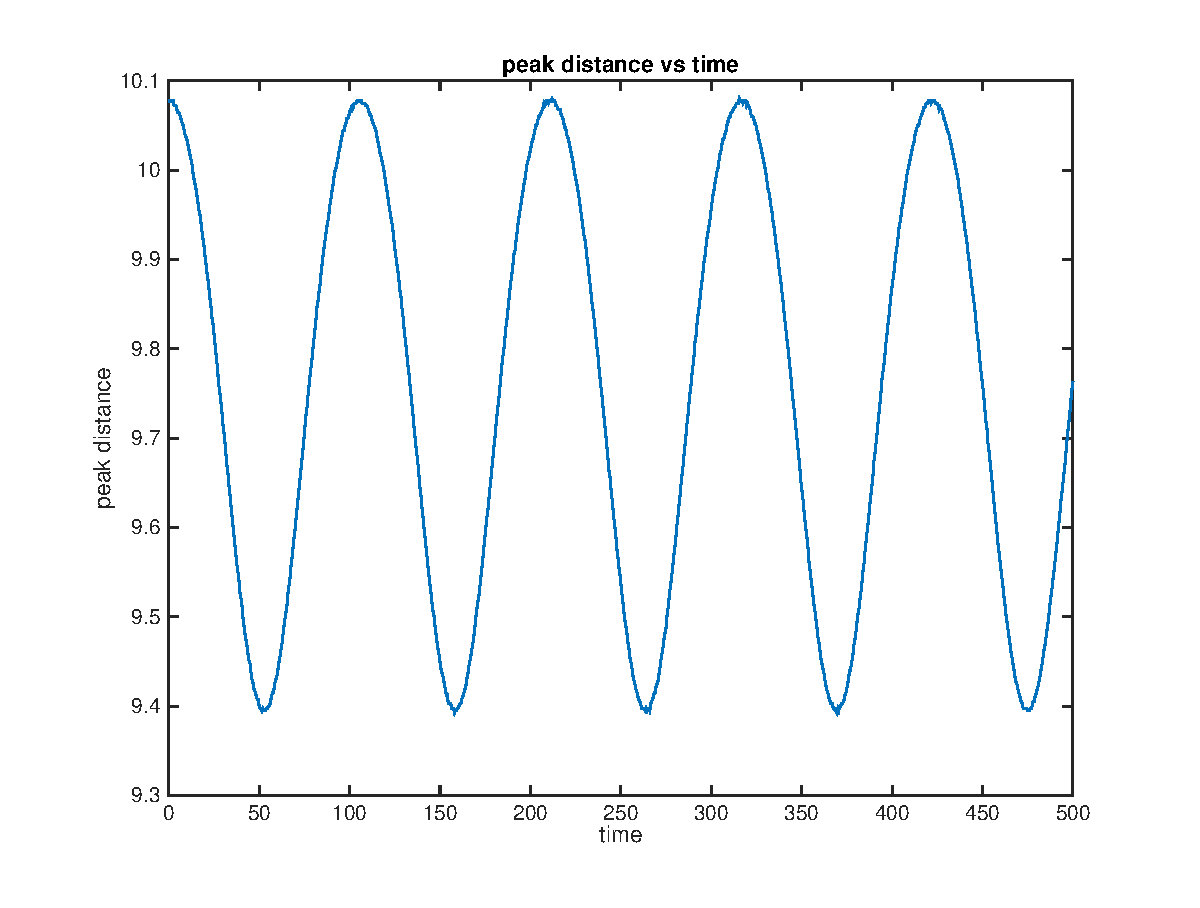
\includegraphics[width=8.5cm]{peakdistvstime}
	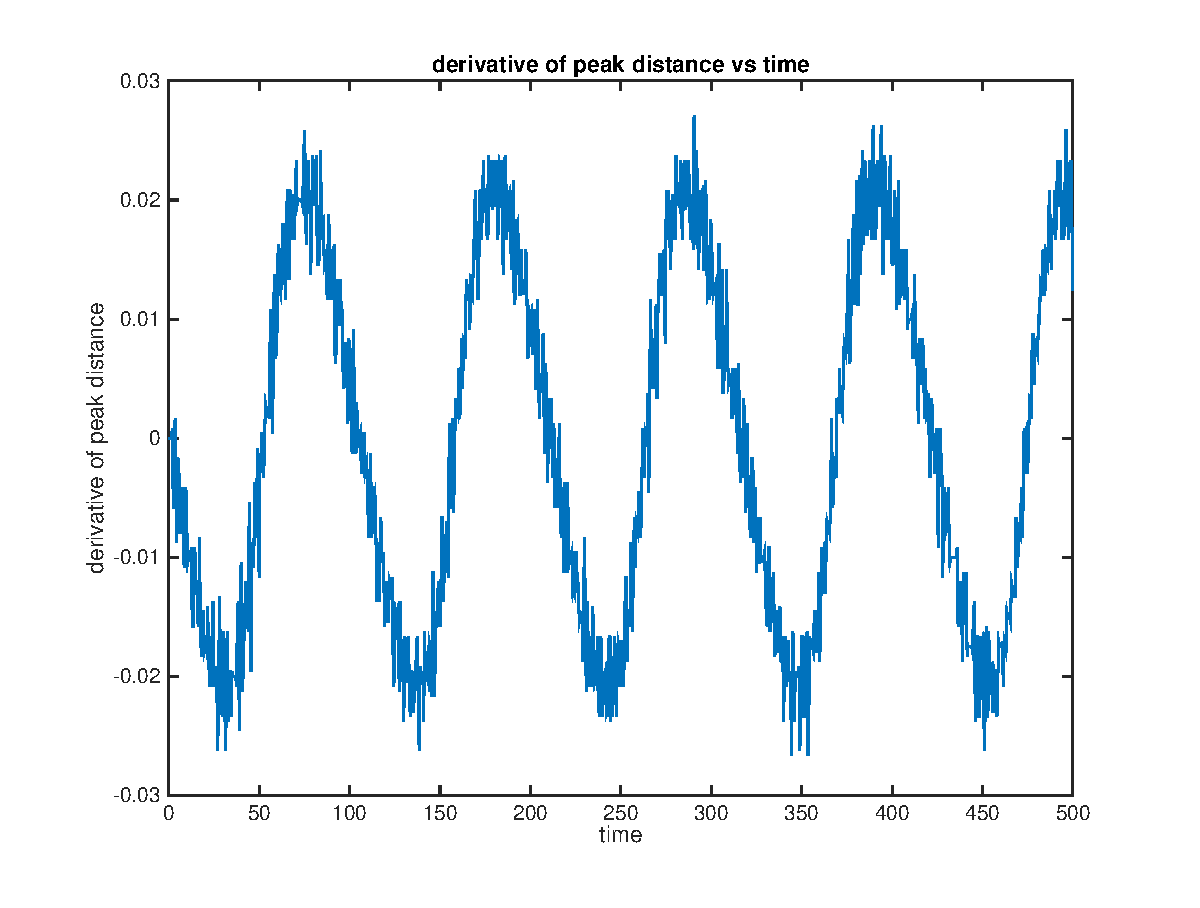
\includegraphics[width=8.5cm]{peakderivvstime}
\end{figure}

Another way we could do this is to look at the heights of the two peaks. Peak height and wave velocity are linearly related, as we showed above. The heights of the two peaks change as the peak distance oscillates, so we should be able to compute the derivative of the peak distance (how fast the peak distance is changing) using the difference between the two peak heights. Using our linear relation above, if we divide the peak height distance by 1.3428, we should get the velocity. We plot this below along with the peak distance derivative. They match up very well, which is good.
\begin{figure}[H]
	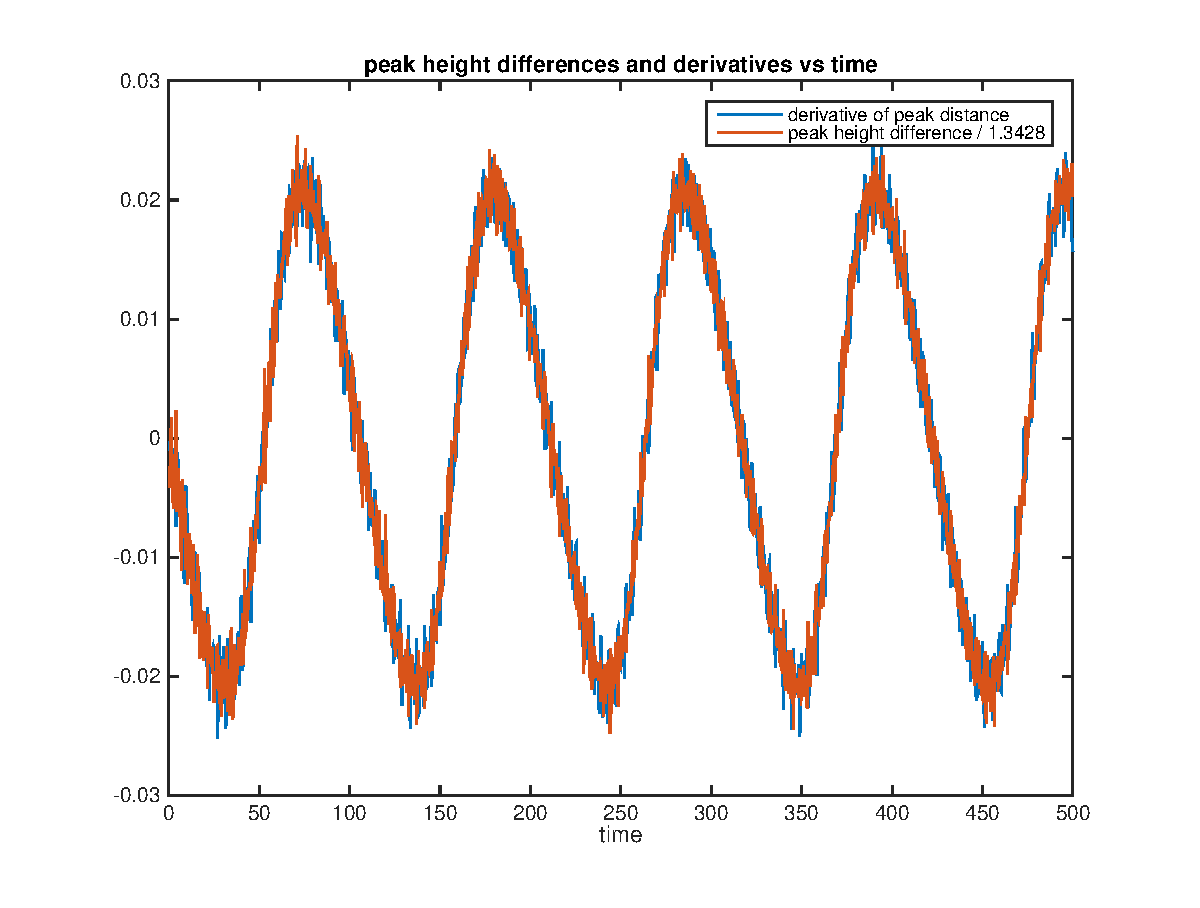
\includegraphics[width=8.5cm]{peakhtdiff}
\end{figure}
However, they are both equally noisy, so I see no reason to use the peak height difference method over taking the derivative using finite differences.\\

The peak distance plot looks fairly smooth, but there are a lot of high-frequency small-amplitude oscillations which are picked up in the plot of the derivative. If we plot peak distance vs peak derivative as time progresses, the plot looks like a periodic orbit, but it is fairly noisy.

\begin{figure}[H]
	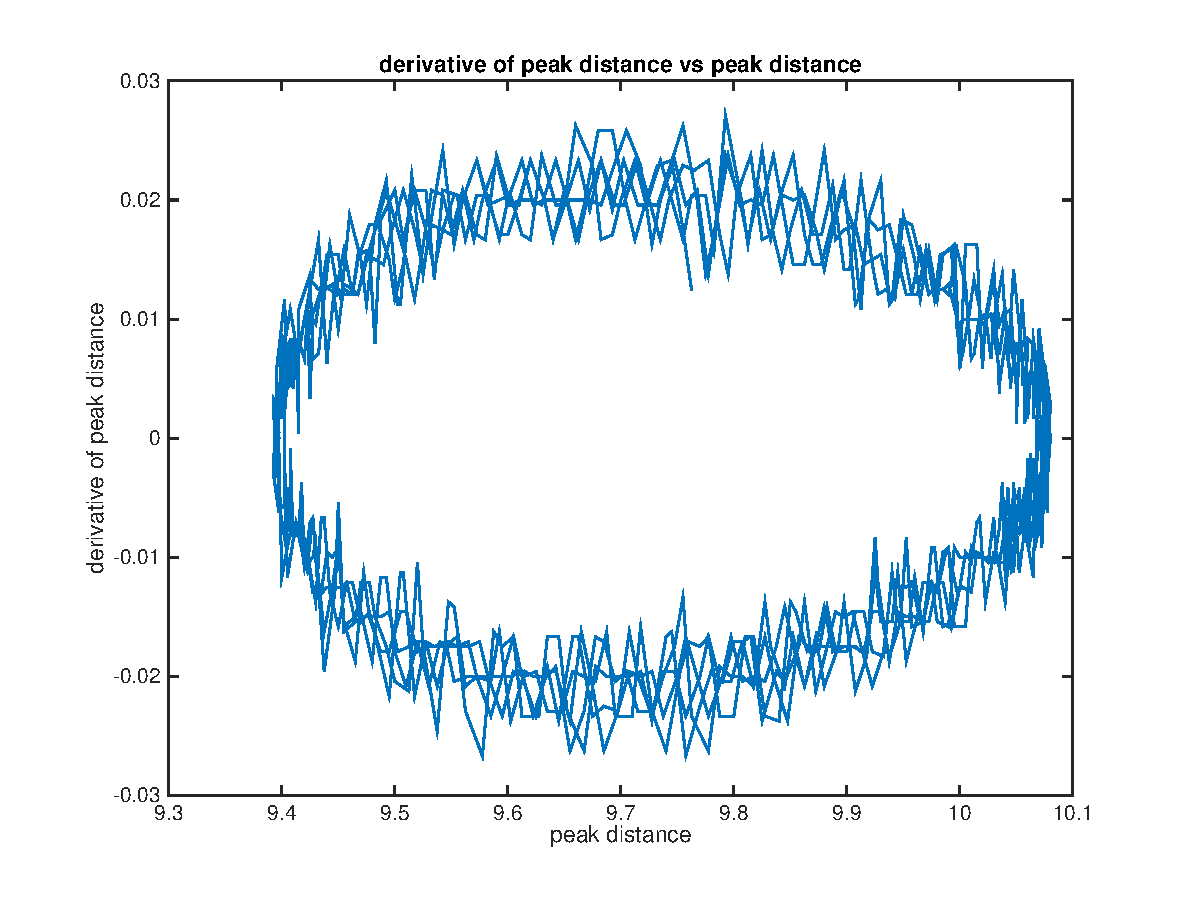
\includegraphics[width=8.5cm]{peakderivdist}
\end{figure}

Using a larger derivative stencil does not improve this, nor does using more Fourier grid points. A small improvement is gained by using Fourier interpolation instead of a cubic spline. In other words, instead of interpolating a spline onto a finer grid, we are finding the interpolating trigonometric polynomial using FFT and finding the zeros of that using Newton's method. This has the advantage that it does not depend on a finer grid. Also it is consistent with the Fourier spectral methods we are using.

\begin{figure}[H]
	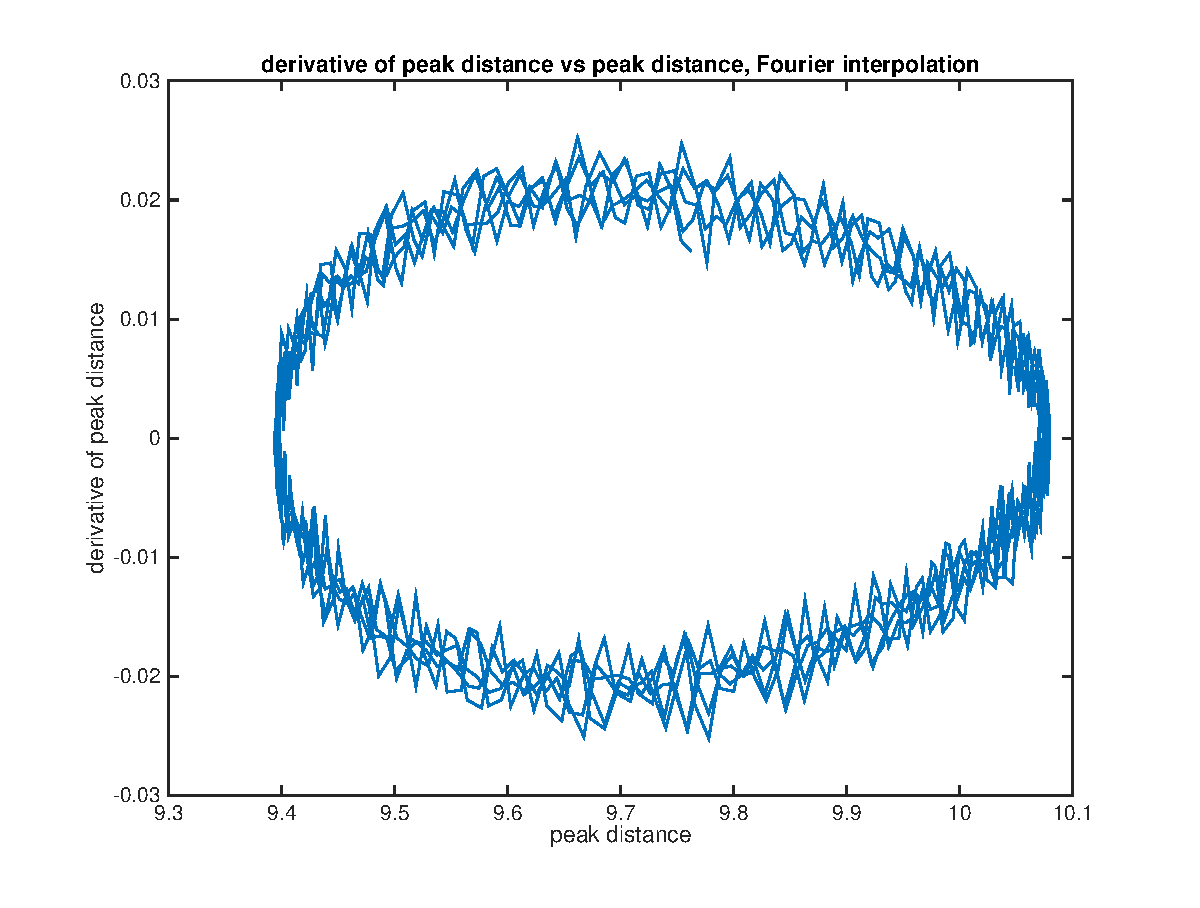
\includegraphics[width=8.5cm]{peakderivdistF}
\end{figure}

Since our data consists primarily of low frequency oscillations and we don't want the high frequency modes, we can smooth the data using the FFT and eliminating all high frequency oscillations. Macroscopically, the plots looks almost identical before and after smoothing, which is good. Here is that comparison plot.

\begin{figure}[H]
	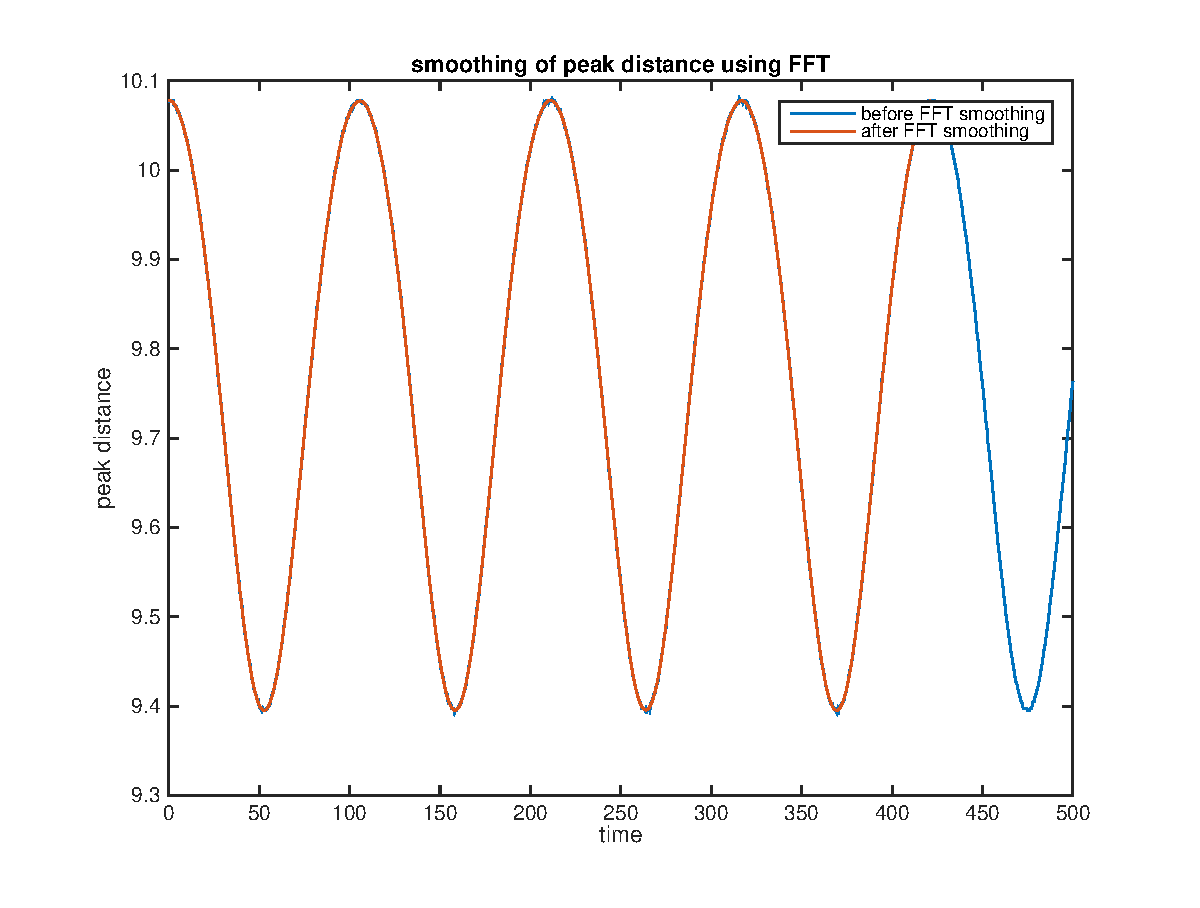
\includegraphics[width=8.5cm]{FFTsmooth}
\end{figure}

Plotting the derivative of the peak distance versus peak distance, after we perform FFT smoothing, we get a much nicer looking periodic orbit. We have four complete cycles in this plot, so it is likely that it is in fact a periodic orbit.

\begin{figure}[H]
	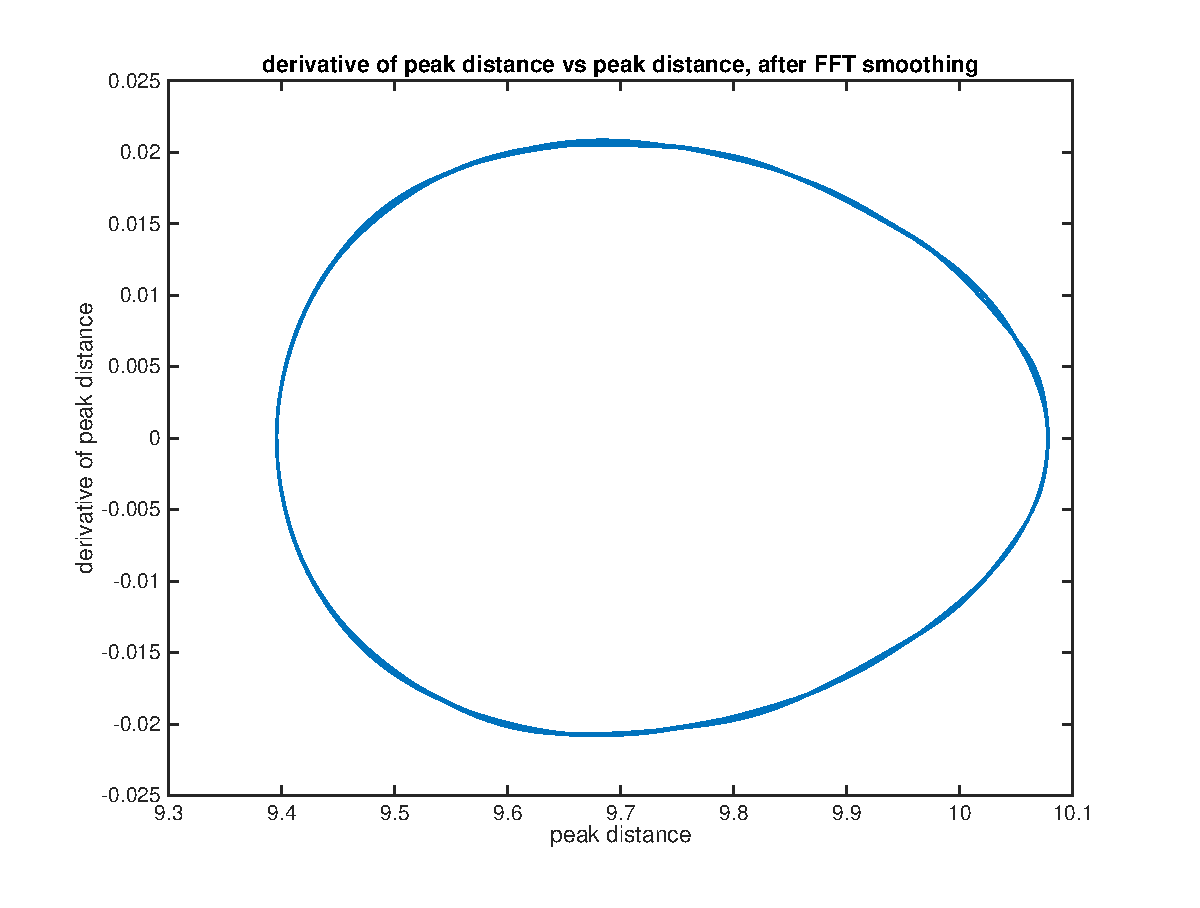
\includegraphics[width=8.5cm]{peakderivdistsmooth}
\end{figure}

\pagebreak

We can take all of this and plot a phase portait of our system. We use solutions near Double Pulses 1, 2, 3, and 4. We expect 1 and 3 to be saddles (marked X) and 2 and 4 centers (marked with a dot). Periodic orbits are smoothed using FFT. Nonperiodic trajectories are smoothed using a moving window filter. The phase portait using all our data is shown here.
\begin{figure}[H]
	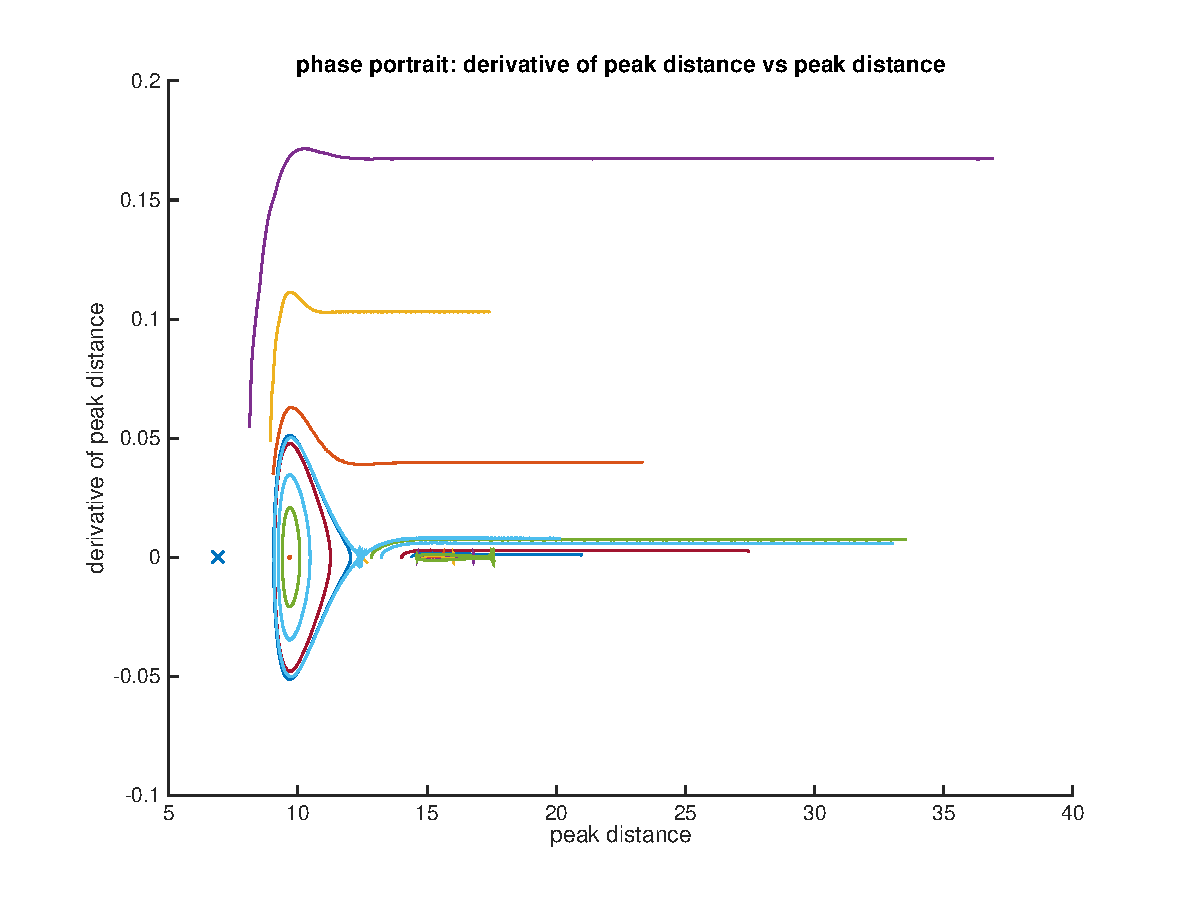
\includegraphics[width=17cm]{phase1}
\end{figure}

\pagebreak

Zooming in on the center around Double Pulse 2, we can see an approximation of a homoclinic orbit starting at the saddle associated with Double Pulse 3.
\begin{figure}[H]
	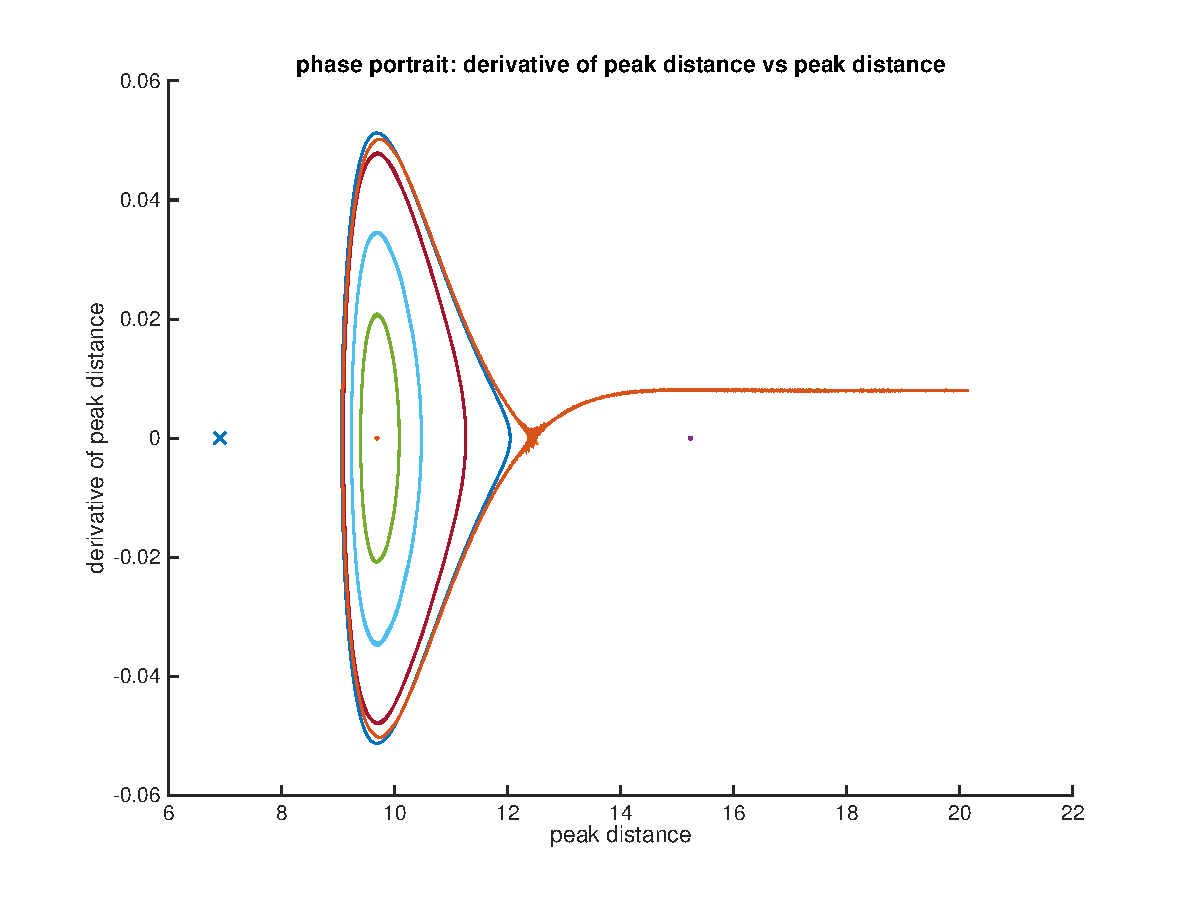
\includegraphics[width=17cm]{phase2}
\end{figure}

\pagebreak

Next we zoom in around Double Pulses 3 and 4. This looks like a smaller version of the phase portait around Double Pulses 1 and 2.

\begin{figure}[H]
	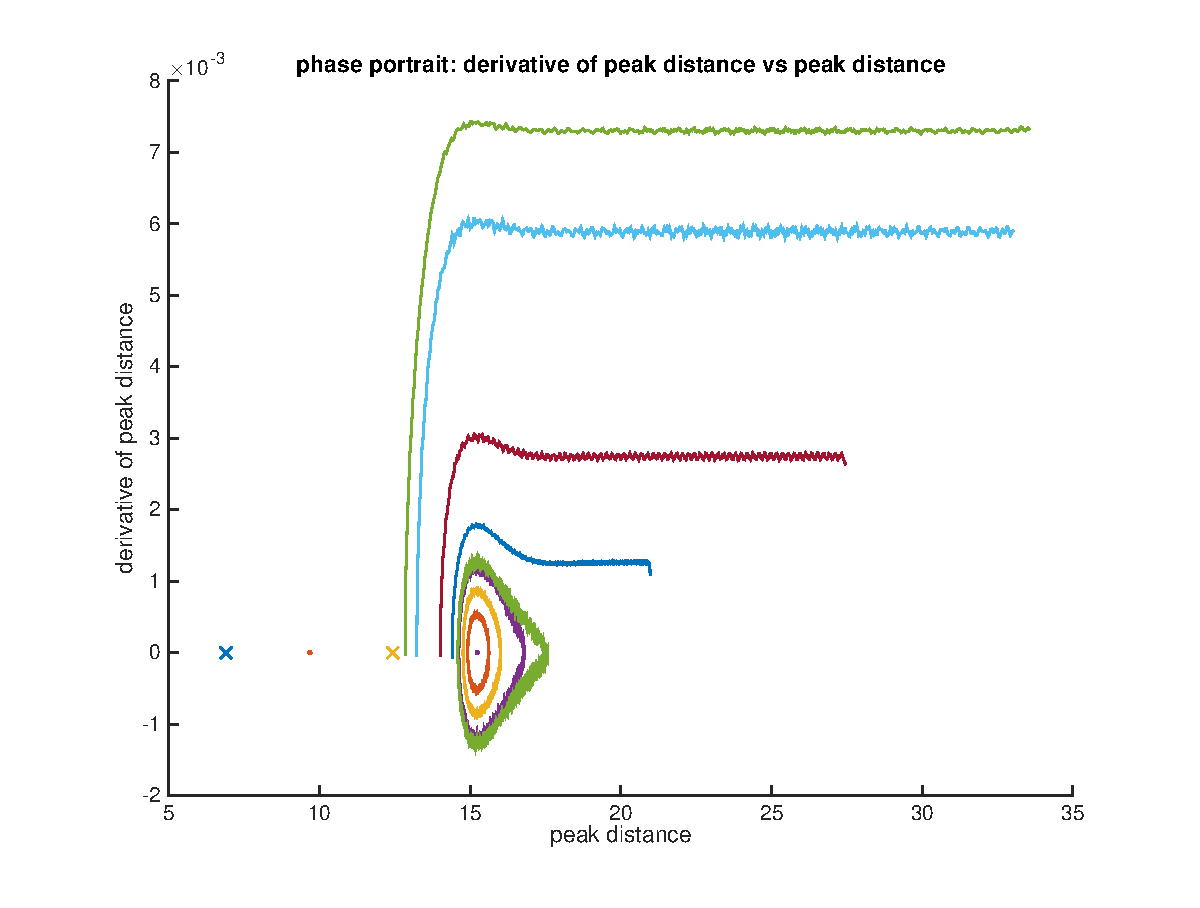
\includegraphics[width=17cm]{phase3}
\end{figure}

\pagebreak

Finally, we zoom in around the center for Double Pulse 4. The amplitude of oscillations in the derivative is much smaller here, and we did less smoothing, but it still looks like a small version of the center for Double Pulse 2.

\begin{figure}[H]
	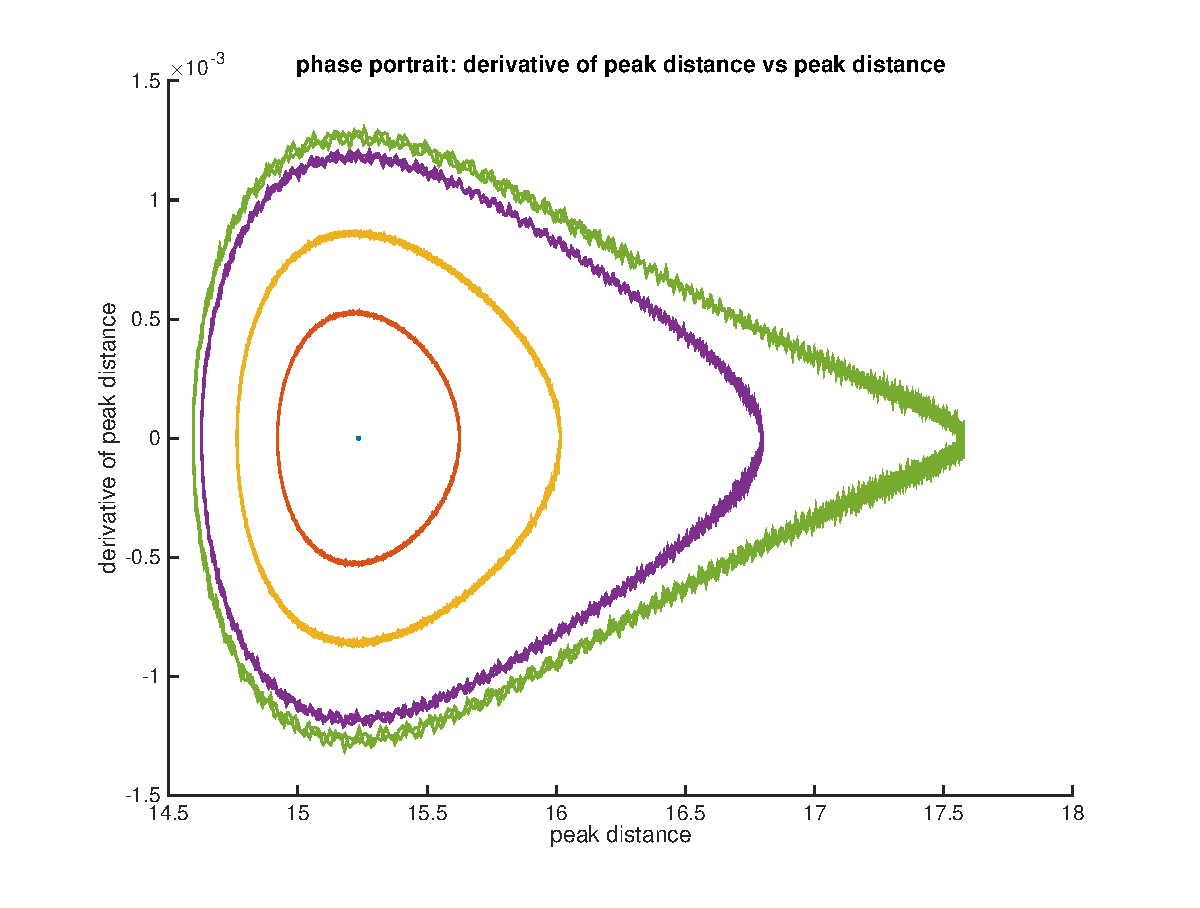
\includegraphics[width=17cm]{phase4.eps}
\end{figure}

Another interesting thing to look at is the relationship between the frequency of oscillations and the amplitude of oscillations (in the peak distance direction) about the two centers. For the frequency, we take $2 pi / T$, where $T$ is the period of oscillations. Plotting this for the two centers, we get:

\begin{figure}[H]
	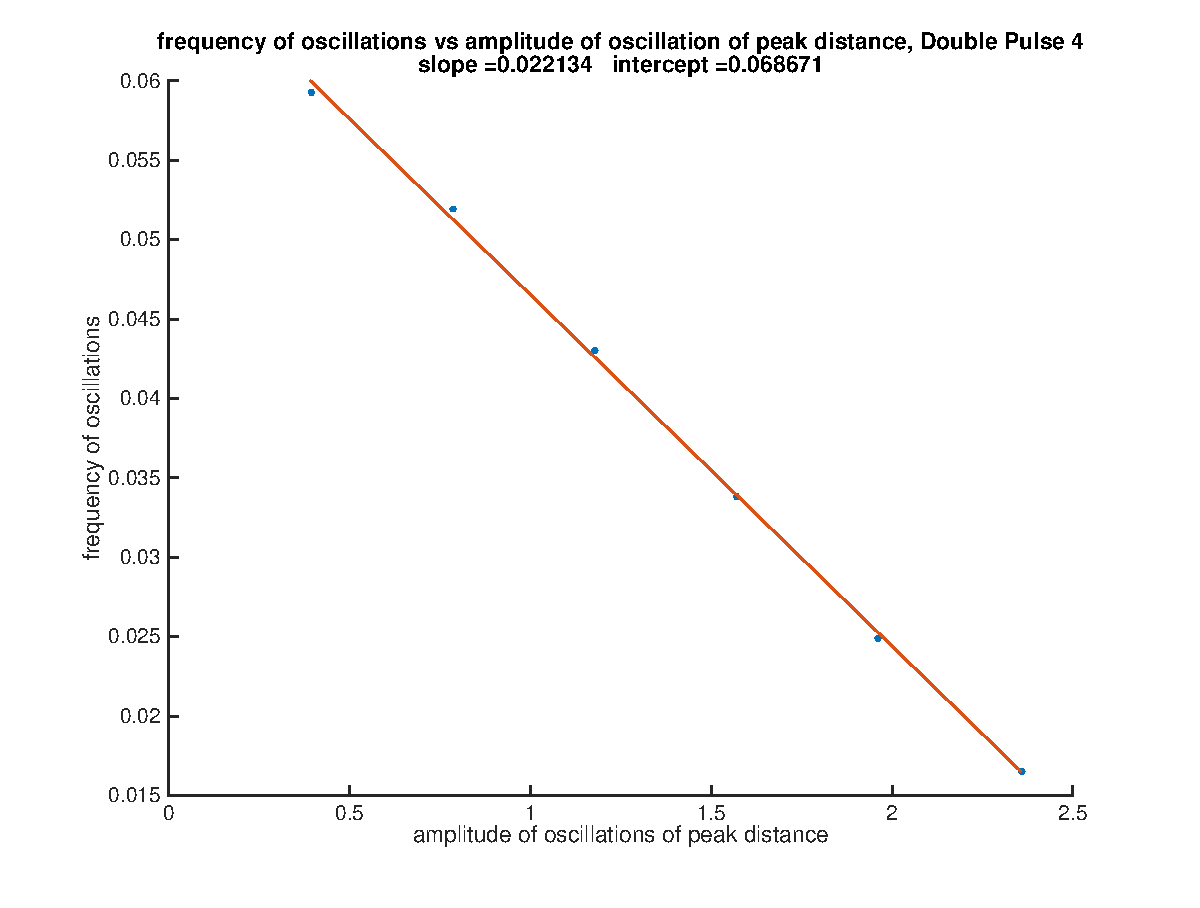
\includegraphics[width=8.5cm]{ampDP2}
	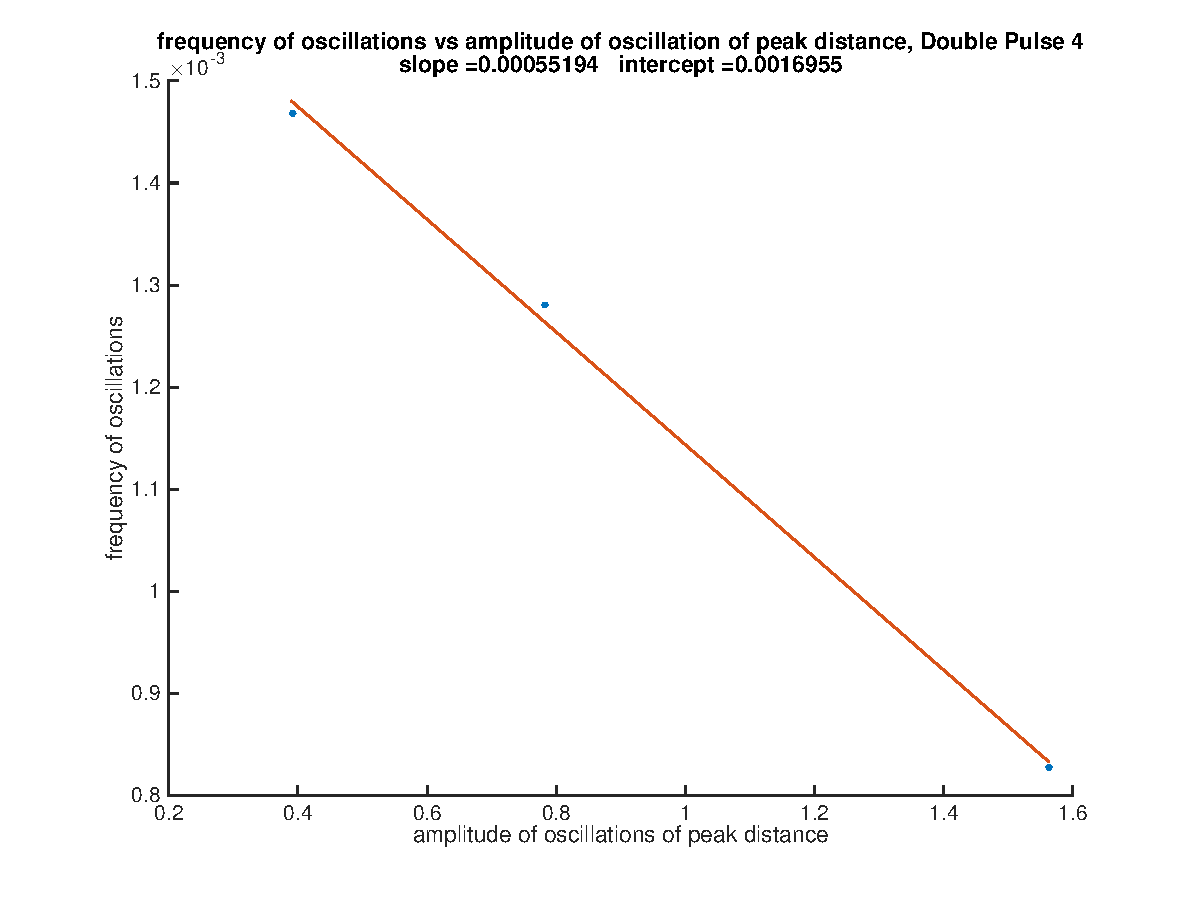
\includegraphics[width=8.5cm]{ampDP4}
\end{figure}

In both cases, we get a good fit straight line. If we extrapolate back to an amplitude of 0 (i.e. take the y-intercept) we get 0.068671 and 0.0016955. These are close to the eigenvalues of 0.0629 and 0.0015 (about 10 percent off in both cases). It is possible that with more data points we would get closer.


\end{document}